\documentclass[../../main.tex]{subfiles}

 \lhead{Implementation: Real RIR Measurements}
 
\begin{document}

\section{Implementation}
	This section describes the steps taken from setting the project objectives to reaching the final implementation of the desired system.


\subsection{Real RIR Recordings}
	In order to test the perceptual differences when using synthetic RIRs, real RIRs of the same space had to be taken.

	To analyse the \ac{VSS} in the past 

	Previous test in the VSS have required ‘Plausibility’ test, where the user must evaluate the response of the VSS without reference to the real venue. This is usually because testing a virtual environment against a real one (authenticity tests) requires travel which can be expensive and difficult. Therefore, by running test based on ‘plausibility’ a sense of how convincing the virtual room is can be obtained. In the case of other virtual reality systems where the virtual environment does not exist in the real world, only these types of test can be run.

	Though plausibility test are acceptable, an authenticity test gives more objective results. Therefore impulse responses of Hendrix Hall were taking, in the same format as the synthesised RIR’s.

	B-Format ambisons RIRs were taken using a B-format soundfield microphone, a Genelec 8040B all at a height of [Enter height] in a number of positions around the room in 4 directions for each.


	\subsubsection{RIR Measurement Setup}

		For the \ac{VSS} it is desirable to obtain \ac{RIR}'s that can be used to represent the topology of a singer, i.e mouth (sound source) bellow the ears (receiver). For this application it is more appropriate to use a Head and Torso simulator, however due to the unavailability of such equipment, a Genelec 8040B \cite{genelec} loudspeaker was used as a directional sound source instead and a Soundfield microphone was used as the receiver.

		Figure~\ref{realRIRTop} shows the \ac{RIR} measurement set up with the Genelec placed 1m above the ground and the Soundfield microphone places 0.6m above the sound source. Ideally the receiver would be placed closer to the sound source to more accurately represent the distance between the ears and the mouth, however due to the physical dimensions of the equipment being used this was not possible. The sound source was placed 1m off the ground simply due to the limitations set by the maximum height of the microphone stand.

		\begin{figure}
			\begin{center}
				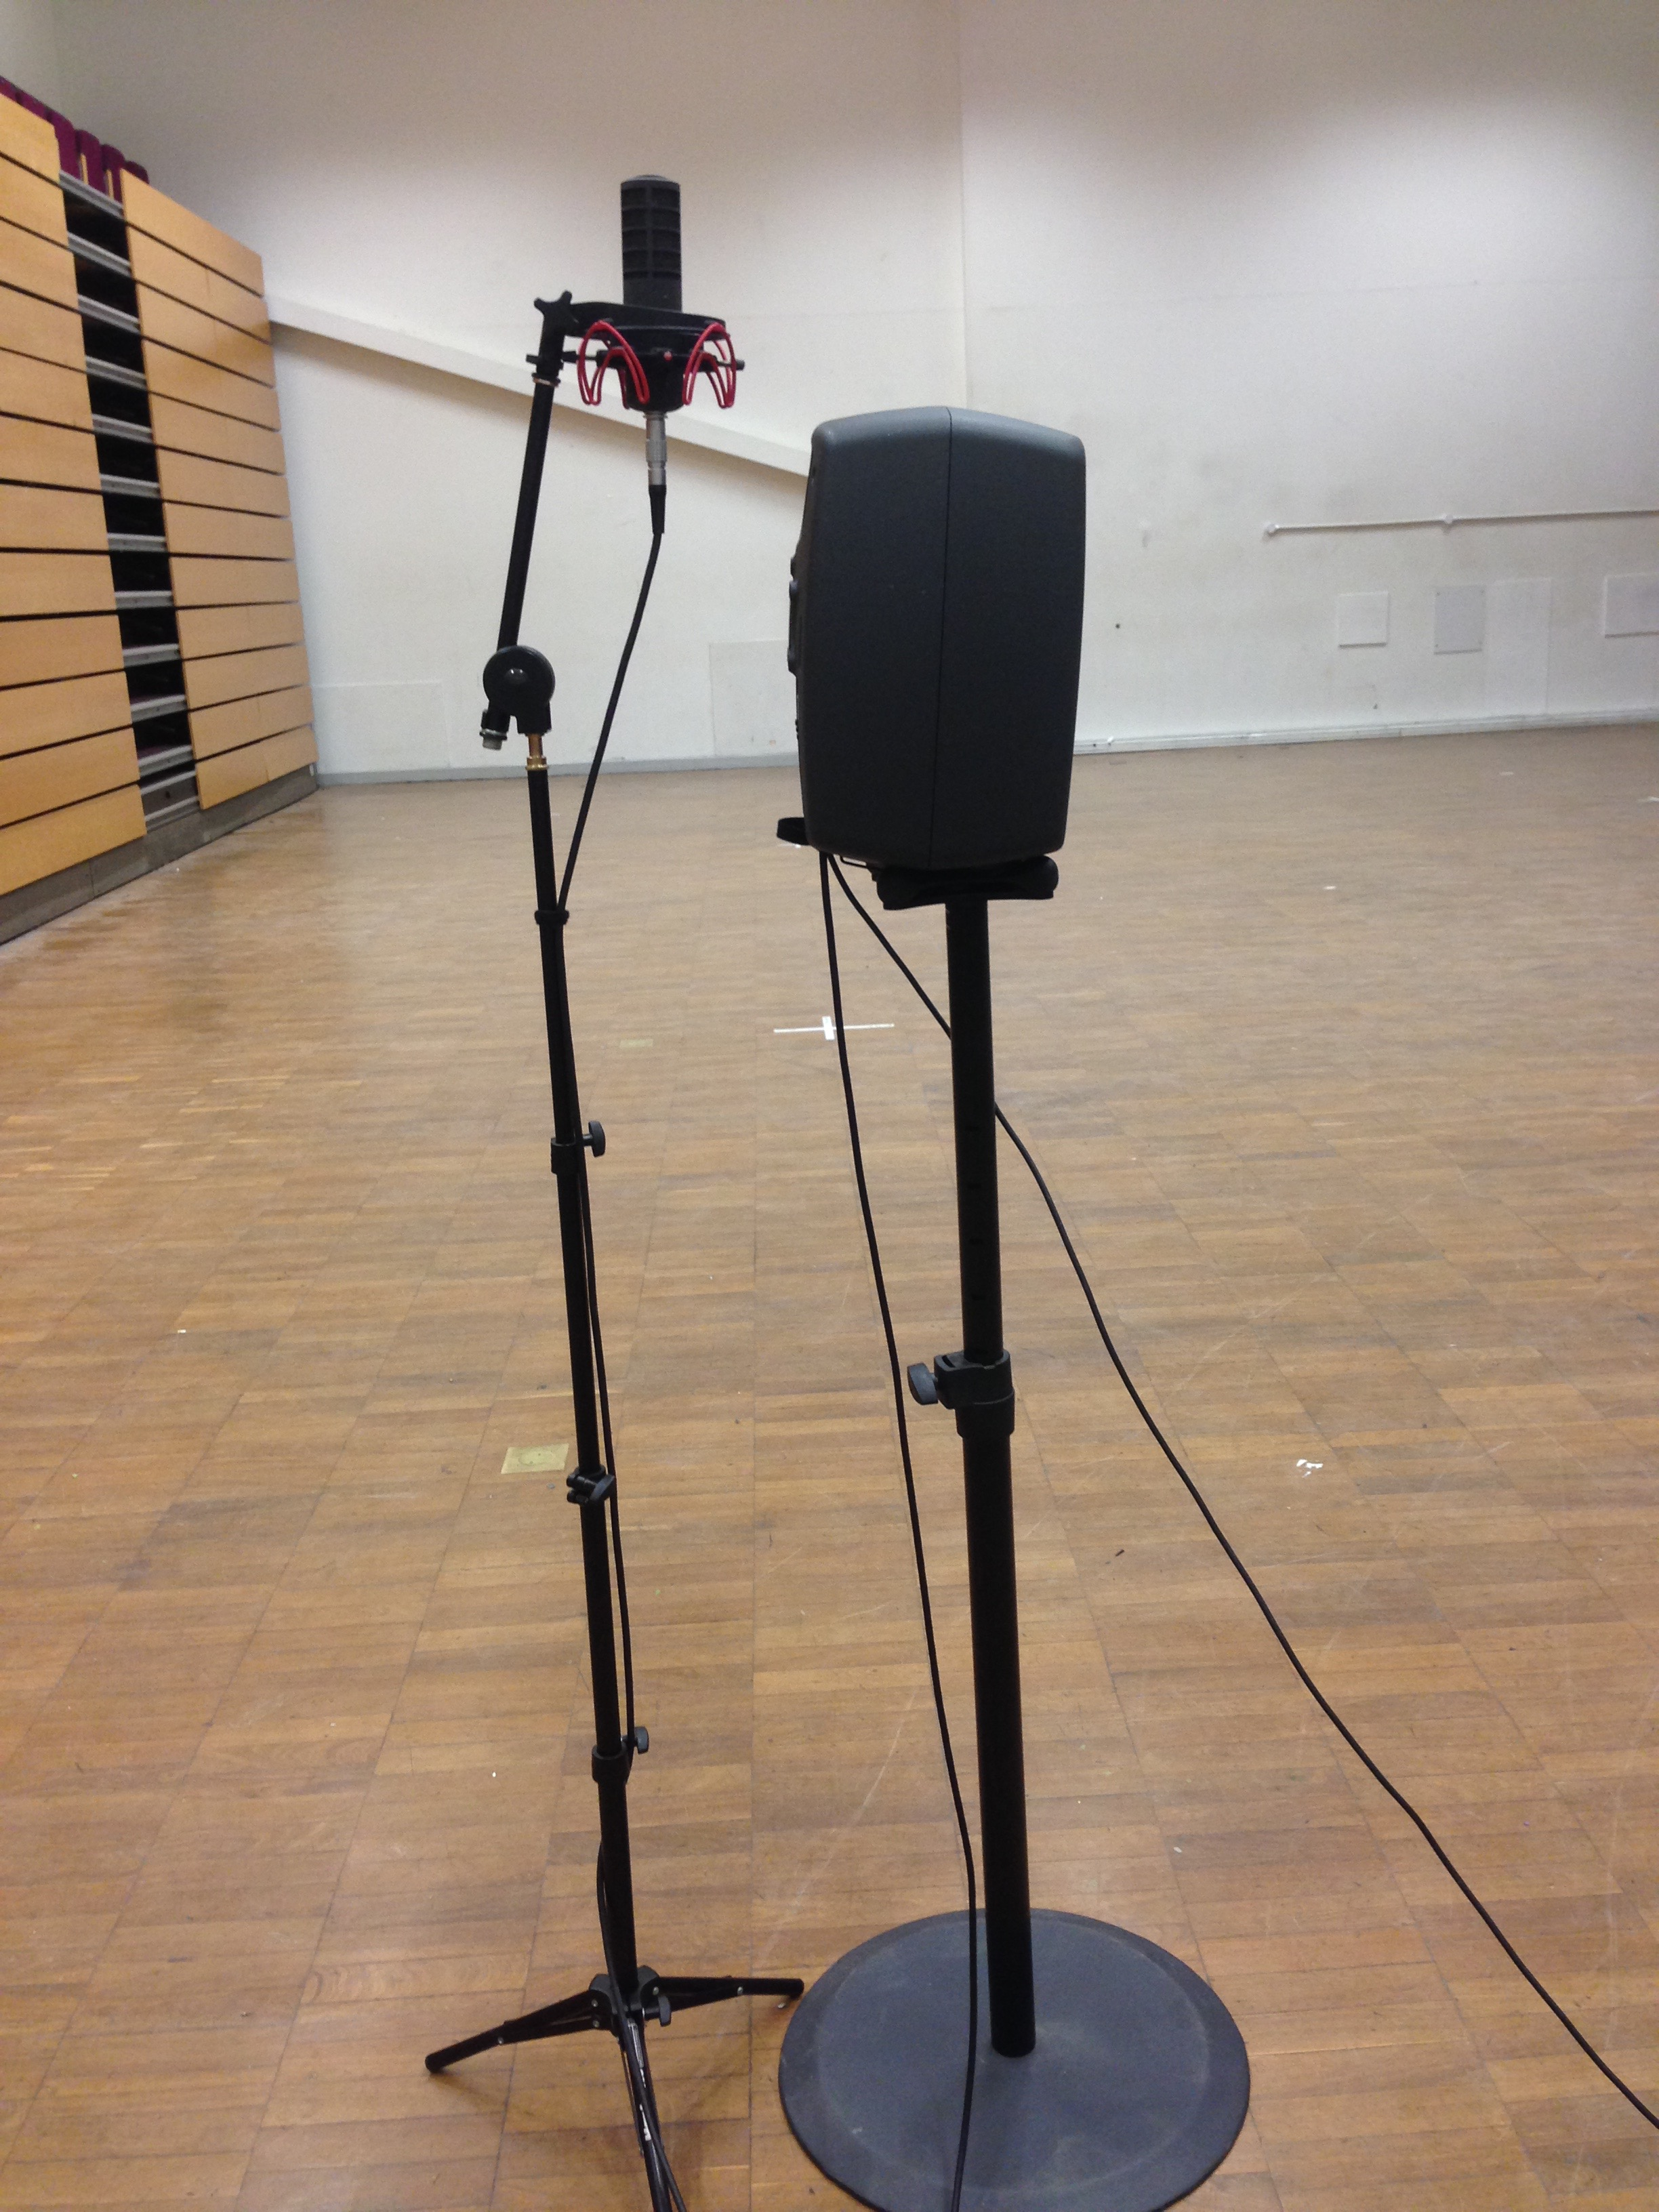
\includegraphics[scale = 0.1]{Sections/Implementation/RealRIRs/images/realRIRTopology1.jpg} 
				\caption{Human head topology \ac{RIR} measurement set up with a Genelec 8040B sound source placed 1m off the floor 0.6m below a Soundfield microphone used as a receiver}
				\label{realRIRTop}
			\end{center}
		\end{figure}

	\subsubsection{Positions}

		Four positions within the room were chosen for the \ac{RIR} positions shown in figure~\ref{rirPositions} where:

		\begin{center}
			\begin{tabular}{l| c c c c}
				Position & (1) & (2) & (3) & (4) \\
				Coordinates [x,y] (m) & [9,9] & [4.5,9] & [2,9] &  [10.13,1.46]\\
			\end{tabular}
		\end{center}


		\begin{figure}
			\begin{center}
				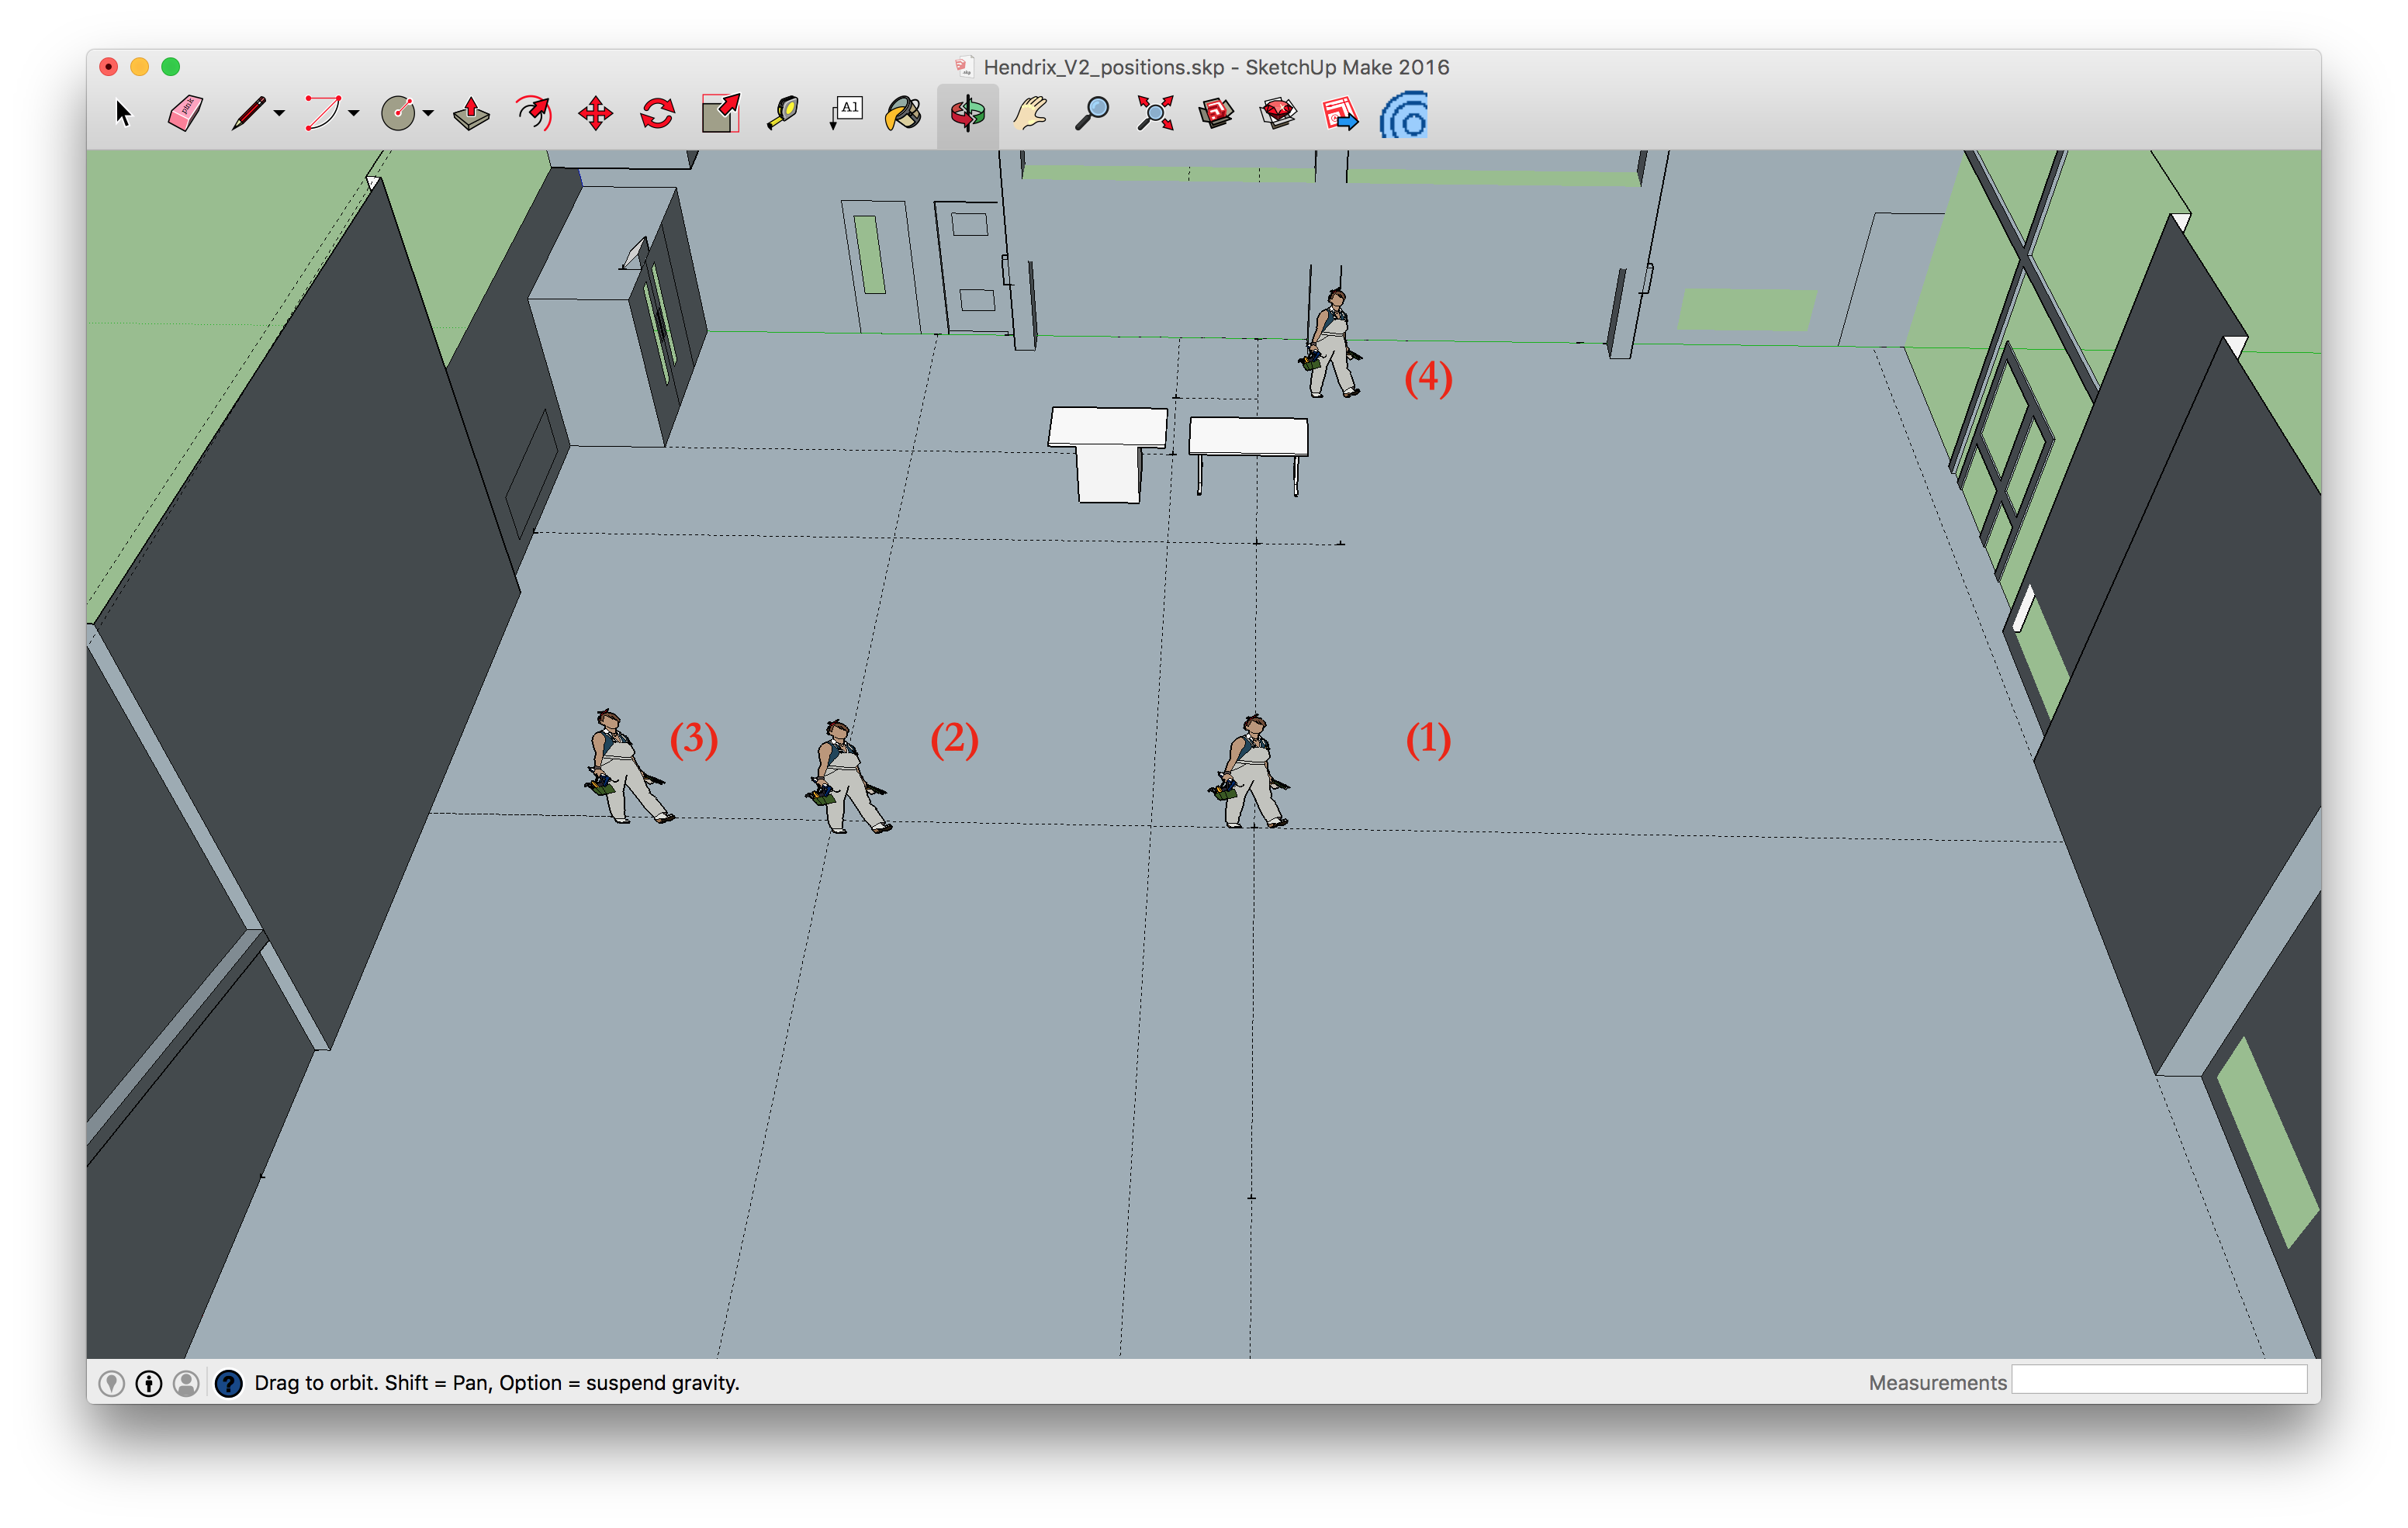
\includegraphics[scale = 0.3]{Sections/Implementation/RealRIRs/images/Real_RIRs7_edit.png} 
				\caption{Google SketchUp model showing the positions of where the real \ac{RIR}'s were taken}
				\label{rirPositions}
			\end{center}
		\end{figure}

		
		
	\subsubsection{RIR Analysis}

	\subsubsection{Issues: False Start}
		Simple wiring error

\end{document}